\documentclass[fleqn]{beamer}
\beamertemplatenavigationsymbolsempty

\usepackage[T1]{fontenc}
\usepackage[utf8]{inputenc}

\usepackage{amsmath,amssymb}
\usepackage{graphicx}
\usepackage{mathptmx}
\usepackage{subcaption}
\usepackage{amsthm}
\usepackage{tikz}
%\usepackage[colorlinks=true,naturalnames=true,plainpages=false,pdfpagelabels=true]{hyperref}
\usetikzlibrary{patterns,decorations.pathmorphing,positioning, arrows, chains}

\usepackage[backend=biber, sorting=none]{biblatex}
\addbibresource{cite.bib}

\setbeamertemplate{endpage}{%
    \begin{frame}
        \centering
        \Large \emph{Thank You!}
    \end{frame}
}

\AtEndDocument{\usebeamertemplate{endpage}}

% vertical separator macro
\newcommand{\vsep}{
  \column{0.0\textwidth}
    \begin{tikzpicture}
      \draw[very thick,black!10] (0,0) -- (0,7.3);
    \end{tikzpicture}
}
\setlength{\mathindent}{0pt}

% Beamer theme
\usetheme{UniVienna}
\usefonttheme[onlysmall]{structurebold}
\mode<presentation>
\setbeamercovered{transparent=10}

\title
{SGD with Large Step Sizes Learns Sparse Features}
\subtitle{Seminar Optimization}
\author[Popović Milutin]
{Popović Milutin\newline\newline Supervisor: Radu Ioan Bot}
\date{23. January 2024}

\begin{document}
    \begin{frame}
        \maketitle
    \end{frame}

    \begin{frame}{Introduction SGD}
        \begin{itemize}[<+->]
        \item[] Given:
            \begin{itemize}
                \item input/output samples $(x_i, y_i)_{i=1}^{n} \in
                    \mathbb{R}^{d} \times \mathbb{R}$
                \item Prediction functions
                    $\mathcal{H} = \{x \mapsto h_{\theta}(x)\; | \; \theta \in
                    \mathbb{R}^{p}\}$
                \item setting $p \gg n$
            \end{itemize}
        \item[] Minimize the loss function
        \begin{center}
            \begin{minipage}{0.5\textwidth}
                \begin{align*}
                    \mathcal{L}(\theta) := \frac{1}{2n} \sum_{i=1}^{n} \left(
                    h_\theta(x_i) - y_i \right)^{2},
                \end{align*}
            \end{minipage}
        \end{center}
        \begin{itemize}
            \item using Stochastic Gradient Descend (SGD).
        \end{itemize}

    \end{itemize}
    \end{frame}

    \begin{frame}{Introduction SGD}

        \begin{itemize}[<+->]
            \item Instead of computing the gradient of each function in the
                sum \item consider $i \sim U(\{1,\ldots,n\} )$ uniformly distributed with
            \item SGD recursion for learning rate $\eta > 0$, initial $\theta_0
                \in \mathbb{R}^{p}$, $\forall t \in \mathbb{N}$
        \begin{center}
            \begin{minipage}{0.5\textwidth}
                \begin{align*}
                    \theta_{t+1} = \theta_t - \eta\left(h_{\theta_t}(x_{i_t})
                    - y_{i_t}\right)
                    \nabla_{\theta} h_{\theta_t}(x_{i_t}).
                \end{align*}
            \end{minipage}
        \end{center}
        \end{itemize}

    \end{frame}


    \begin{frame}{GD with specific Label Noise}
        \begin{itemize}[<+->]
            \item Define a random vector $\xi_t \in \mathbb{R}^{n}$ in each iteration
                $t \ge 0$
                \begin{center}
                \begin{minipage}{0.5\textwidth}
                    \begin{align*}
                        [\xi_t]_i := (h_{\theta_t}(x_i) -
                        y_i)(1-n\mathbf{1}_{i=i_t})
                    \end{align*}
                \end{minipage}
                \end{center}
                \vspace{0.5cm}
            \item Then $(\theta_t)_{t\ge0}$ follows the full-batch gradient
                dynamics on $\mathcal{L}$
                \begin{center}
                \begin{minipage}{0.5\textwidth}
                \begin{align*}
                    \theta_{t+1} = \theta_t - \frac{\eta}{n} \sum_{i=1}^{n}
                    \left( h_{\theta_t}(x_i) - y_i^{t} \right)
                    \nabla_{\theta} h_{\theta_t}(x_i),
                \end{align*}
                \end{minipage}
                \end{center}
                where $y^{t}:= y + \xi_t$.
            \item Note: $\xi_t$ is mean zero r.v.
            \item Note: Variance of $\xi_t$ is
                $\frac{1}{n(n-1)}\mathbb{E}\|\xi_t\|^{2} = 2
                \mathcal{L}(\theta_t)$.
        \end{itemize}
    \end{frame}

    \begin{frame}{GD with specific Label Noise}
        \begin{center}
        \begin{minipage}{0.5\textwidth}
            \begin{align*}
                \theta_{t+1} = \theta_t - \frac{\eta}{n} \sum_{i=1}^{n}
                \left( h_{\theta_t}(x_i) - y_i^{t} \right)
                \nabla_{\theta} h_{\theta_t}(x_i),
            \end{align*}
        \end{minipage}
        \end{center}
        \begin{itemize}
            \item The noisy part at state $\theta$ belongs to the space
                spanned by $\{\nabla_\theta
                h_\theta(x_1),\ldots,\nabla_\theta h_\theta(x_n)\} $
            \item During loss stabilization of large step sizes: may lead to
                a constant effective scale of label noise.
        \end{itemize}
    \end{frame}

    \begin{frame}{Quadratic Loss Stabilization}
        \begin{itemize}[<+->]
            \item Non-convex toy model:
            \item One-dimensional data $x_i$ from distribution $\hat{\rho}$
            \item linear model outputs $y_i = x_i \theta_*^{2}$
            \item Quadratic loss $F(\theta) :=
                \frac{1}{4}\mathbb{E}_{\hat{\rho}}(y-x\theta^{2})^{2}$ with
                SGD recursion for $\eta > 0$, $t \in \mathbb{N}$:
        \begin{center}
        \begin{minipage}{0.5\textwidth}
            \begin{align*}
                \theta_{t+1} = \theta_t + \eta \theta_t x_{i_t}(y_{i_t} -
                x_{i_t}\theta^{2}_t)
            \end{align*}
        \end{minipage}
        \end{center}


        \end{itemize}

    \end{frame}

    \begin{frame}{Quadratic Loss Stabilization}
        \begin{block}{\textbf{Proposition:} Loss Stabilization}
            Assume $\exists x_{\text{min}}, x_{\text{max}} > 0$ s.t.
            $\text{supp}(\hat{\rho}) \subset [x_\text{min}, x_\text{max}]$.
            Then for any $\eta \in \left( (\theta_* x_\text{min})^{-2}, 1.25
            (\theta_*x_\text{max})^{-2}\right)$, any initial $\theta_{0} \in
            (0, \theta_*)$, for all $t \in \mathbb{N}$ we have that
            \textbf{almost surely}
            \begin{center}
            \begin{minipage}{0.5\textwidth}
            \begin{align*}
                F(\theta_t) \in \left(\varepsilon_0 \theta_*^{2},\; 0.17
                \theta_*^{2}\right),
            \end{align*}
            \end{minipage}
            \end{center}
        where $\varepsilon_0 := \min
        \{\frac{\eta(\theta_*x_\text{min})^{2}-1}{3},\; 0.02\}$.
        \newline
        And \textbf{almost surely} there exists $t, k >0$ s.t.
        \begin{center}
        \begin{minipage}{0.5\textwidth}
        \begin{align*}
            &\theta_{t+2k} \in (0.65\theta_*, (1-\varepsilon_0)\theta_*) \quad
            \text{and}\\
            &\theta_{t+2k+1} \in ((1-\varepsilon_0)\theta_*, 1.162\theta_*)
        \end{align*}
        \end{minipage}
        \end{center}
        \end{block}
    \end{frame}

    \begin{frame}{Quadratic Loss Stabilization}
        \begin{itemize}[<+->]
            \item For clarity rescale $\theta_t \to \theta_t/\theta_*$
            \begin{center}
            \begin{minipage}{0.5\textwidth}
                \begin{align*}
                    \theta_{t+1} = \theta_t + \gamma\theta_t\left(
                    1-\theta_t^{2} \right),
                \end{align*}
            \end{minipage}
            \end{center}
            where $\gamma \sim \hat{\rho}_{\gamma}$ is the pushforward
            $\hat{\rho}$ under $z \mapsto \eta\theta_*^{2}z^2$.

        \item then the interval of $\eta$ becomes that of
            $\text{supp}(\hat{\rho}_{\gamma}) \subseteq (1, 1.25)$.
        \end{itemize}
    \end{frame}

    \begin{frame}{Quadratic Loss Stabilization}
        \begin{itemize}[<+->]
            \item To prove the proposition divide $(0, 1.162)$ into 4
                regions
            \item $I_0=(0, 0.65]$, $I_1=(0.65, 1-\varepsilon)$,
                $I_2=[1-\varepsilon, 1)$ and $I_3 = [1, 1.162)$.

            \item All iterates end up in $I_1$, leave and come back to $I_1$
                in 2 steps.

            \item divided into 4 steps
                \begin{enumerate}
                    \item There is a $t\ge 0$: $\theta_t \in I_1\cup
                        I_2\cup I_3$
                    \item For $\theta_t \in I_3$, then $\theta_{t+1} \in I_1
                        \cup I_2$.
                    \item For $\theta_t \in I_2$, then there is a $k>0$:
                    $\forall k' < k$, it holds that $\theta_{t+2k'} \in
                        I_2$ and $\theta_{t+2k} \in I_1$
                    \item For $\theta_t \in I_1$, then $\forall k \ge 0$, it
                        holds that
                        $\theta_{t+2k} \in I_1$ and $\theta_{t+2k+1} \in
                        (1+\varepsilon, 1.162)$.
                \end{enumerate}


        \end{itemize}
    \end{frame}

    \begin{frame}{Quadratic Loss Stabilization}
        \begin{itemize}[<+->]
            \item Proof is divided into 4 steps show
                \begin{enumerate}
                    \item There is a $t\ge 0$: $\theta_t \in I_1\cup
                        I_2\cup I_3$
                    \item For $\theta_t \in I_3$, then $\theta_{t+1} \in I_1
                        \cup I_2$.
                    \item For $\theta_t \in I_2$, then there is a $k>0$:
                        $\forall k' < k$, it holds that $\theta{t+2k'} \in
                        I_2$ and $\theta_{t+2k} \in I_1$
                    \item For $\theta_t \in I_1$, then $\forall k \ge 0$, it
                        holds that
                        $\theta_{t+2k} \in I_1$ and $\theta_{t+2k+1} \in
                        (1+\varepsilon, 1.162)$.
                \end{enumerate}
        \end{itemize}
    \end{frame}

    \begin{frame}{Quadratic Loss Stabilization}
        \begin{itemize}[<+->]
            \item For \textbf{1}: (There is a $t\ge 0: \theta_t \in I_1 \cup
                I_2 \cup I_3)$
            \item Show that the function $h_\gamma(\theta) = \theta -
                \gamma\theta(1-\theta^{2})$ for $\gamma \in (1, 1.25)$ stays
                in $(0, 1.162)$.

        \vspace{0.5cm}

            \item For \textbf{2}: (For $\theta_t \in I_3$, then $\theta_{t+1} \in I_1
                        \cup I_2$.)
            \item For $\theta \in (1, 1.162)$ note $h_\gamma(\theta)$ is linear in $\gamma$ when
                $\theta>1$, decreasing as $\gamma$ increases then \newline
                $0.652 = h_{1.25}(1.162) < h_\gamma(1.162) < h_\gamma(\theta)
                    < h_\gamma(1) = 1$

            \item So $\theta_{t+1} \in I_1 \cup I_2$.


        \vspace{0.5cm}

            \item \textbf{3} \& \textbf{4} are a bit more complicated but can be
                shown also with basic analysis.
        \end{itemize}
    \end{frame}


    \begin{frame}{SGD Dynamics}
        \begin{itemize}[<+->]
            \item To further understand loss stabilization -> assume perfect
                stabilization
            \item Conjecture: \textit{During loss stabilization, SGD is well
                modeled by GD with constant label noise}

            \item Label noise dynamics can be studies with Stochastic
                Differential Equations (SDEs)
        \end{itemize}

    \end{frame}

    \begin{frame}{SGD Dynamics Heuristics}
        \begin{itemize}[<+->]
            \item Heuristics: rewrite SGD iteration, where $V_t(\theta_t, i_t) =
                \sqrt{\eta}\left(\nabla_\theta f(\theta_k) - \nabla
                f_{i_t}(\theta_t)  \right)  $ is $p$-dimensional r.v.
            \begin{center}
            \begin{minipage}{0.5\textwidth}
                \begin{align*}
                    \theta_{t+1} = \theta_t - \eta \nabla f(\theta_t) + \eta
                    V_t(\theta_t, i_t).
                \end{align*}
            \end{minipage}
            \end{center}

        \item Straight forward calculation shows
            \begin{center}
            \begin{minipage}{0.5\textwidth}
                \begin{align*}
                    &\mathbb{E}(V_t|\theta_t) = 0, \\
                    &\text{cov}(V_t, V_t|\theta_t) = \eta \Sigma(\theta_t), \\
                    &\Sigma(\theta_k) :=
                    \mathbb{E}\left(\frac{V_t^{2}}{\eta}\Big|\theta_t \right)
                \end{align*}
            \end{minipage}
            \end{center}
        \end{itemize}
    \end{frame}

    \begin{frame}{SGD Dynamics Heuristics}
        \begin{itemize}[<+->]
            \item Then consider  time-homogeneous It\^o type SDE for $\tau\ge 0$
            \begin{center}
            \begin{minipage}{0.5\textwidth}
                \begin{align*}
                    d\theta_\tau = b(\theta_\tau)d\tau
                    +\sqrt{\eta}\sigma(\theta_\tau)dB_\tau,
                \end{align*}
            \end{minipage}
            \end{center}
            where $\theta_\tau \in \mathbb{R}^{p}$, $B_\tau$ standard p-dim.
            Brownian
            motion, $b:\mathbb{R}^{p} \to \mathbb{R}^{p}$ the drift and
            $\sigma: \mathbb{R}^{p}\to \mathbb{R}^{p\times p}$ the diffusion
            matrix

        \item Apply Euler discretization with step size $\eta$ and
            approximate $\theta_{\tau \eta}$ simply with $\hat{\theta}_{\tau}$
            \begin{center}
            \begin{minipage}{0.5\textwidth}
                \begin{align*}
                    \hat{\theta}_t= \hat{\theta}_t + \eta b(\theta_t)
                    +\eta \sigma(\hat{\theta}_t)Z_t,
                \end{align*}
            \end{minipage}
            \end{center}
            with $Z_t = B_{(\tau+1)\eta} - B_{\tau\eta}$ r.v.

        \item Set $b = -\nabla_\theta f$ and $\sigma(\theta) =
            \Sigma(\theta)^{\frac{1}{2}}$, then
            \begin{center}
            \begin{minipage}{0.5\textwidth}
                \begin{align*}
                    d\theta_\tau = -\nabla f(\theta_\tau)d\tau
                    + (\eta\Sigma(\theta_\tau))^{\frac{1}{2}} dB_t.
                \end{align*}
            \end{minipage}
            \end{center}
        \end{itemize}
    \end{frame}

    \begin{frame}{SGD Dynamics Heuristics}
        \begin{itemize}[<+->]
            \item In our case: we have a loss function $\mathcal{L}$
            \item The noise at state $\theta$ is spanned by
                $\{\nabla_\theta h_\theta(x_1), \ldots, \nabla_\theta
                h(x_n)\} $
            \item Loss stabilization occurs at a level set $\delta > 0$
            \begin{center}
            \begin{minipage}{0.5\textwidth}
                \begin{align*}
                    d\theta_\tau = -\nabla_\theta \mathcal{L}(\theta_\tau)d\tau
                    + \sqrt{\eta\delta}
                    \phi_{\theta_\tau}\left(X\right)^{T}dB_\tau,
                \end{align*}
            \end{minipage}
            \end{center}
            \vspace{0.5cm}
            where $\phi_\theta(X) := [\nabla_\theta
            h_\theta(x_i)^{T}]_{i=1}^{n} \in \mathbb{R}^{n\times p}$ is
            referred to as the Jacobian.
        \end{itemize}
    \end{frame}

    \begin{frame}{Diagonal Linear Networks}
        \begin{itemize}[<+->]
            \item Two layer linear network with only diagonal connections:
            \item Prediction function:
                $h_{u, v}(x) = \langle u, v\odot x\rangle =  \langle u \odot
                v, x\rangle$.
            \item Linear predictor $\beta: = u \odot v \in \mathbb{R}^{d}$
            \item Gradient $\nabla_u h_{u, v}(x) = v \odot x$.
            \item SDE model (symmetric for v)
            \begin{center}
            \begin{minipage}{0.5\textwidth}
                \begin{align*}
                    du_\tau = -\nabla_u \mathcal{L}(u_\tau, v_\tau) d\tau
                    +\sqrt{\eta \delta} v_\tau \odot [X^{T}dB_\tau].
                \end{align*}
            \end{minipage}
            \end{center}

        \end{itemize}
    \end{frame}

    \begin{frame}{Diagonal Linear Networks: Conclusion}
        \begin{itemize}[<+->]
            \item During the first phase SGD with large $\eta$
                \begin{enumerate}
                    \item decreases the training loss
                    \item stabilizes at some level set $\delta$
                \end{enumerate}
            \item Meanwhile there is an effective noise-driven dynamics
                which oscillates on $\mathcal{O}(\sqrt{\eta\delta})$
            \item Decreasing the step size later leads to recovery of the
                sparsest predictor.
        \end{itemize}
    \end{frame}

    \begin{frame}{Sparsity Coefficient}
        \begin{itemize}[<+->]
             \item SDE dynamics of diagonal networks emphasizes that there is
                 a sparsity bias because of $v \odot [X^{T}dB_\tau]$ leading
                 to a coordinate shrinkage effect
            \item Generally the same thing happens w.r.t the Jacobian
                $\phi_\theta(X)$ leading to the same effect.
            \begin{center}
            \begin{minipage}{0.5\textwidth}
                \begin{align*}
                    d\theta_\tau = -\nabla_\theta \mathcal{L}(\theta_\tau)d\tau
                    + \sqrt{\eta\delta}
                    \phi_{\theta_\tau}\left(X\right)^{T}dB_\tau,
                \end{align*}
            \end{minipage}
            \end{center}
            \item Conjecture: SDE noise part minimizes the $l_{2}$-norm of
                the columns of $\phi_\theta(X)$.

            \item Columns can be reduced to zero below a threshold. (fitting
                part does not allow the Jacobian to collapse to zero)
         \end{itemize}
    \end{frame}

    \begin{frame}{DLN Feature Sparsity Coefficient}
        \begin{itemize}[<+->]
            \item The Jacobian can be simplified during loss stabilization.
            \item Motivation: count the average number of distinct, nonzero
                activations over the training set = \textbf{feature sparsity
                coefficient}
        \end{itemize}
    \end{frame}

    \begin{frame}{DLN Results}
        \begin{figure}[htpb]
            \centering
            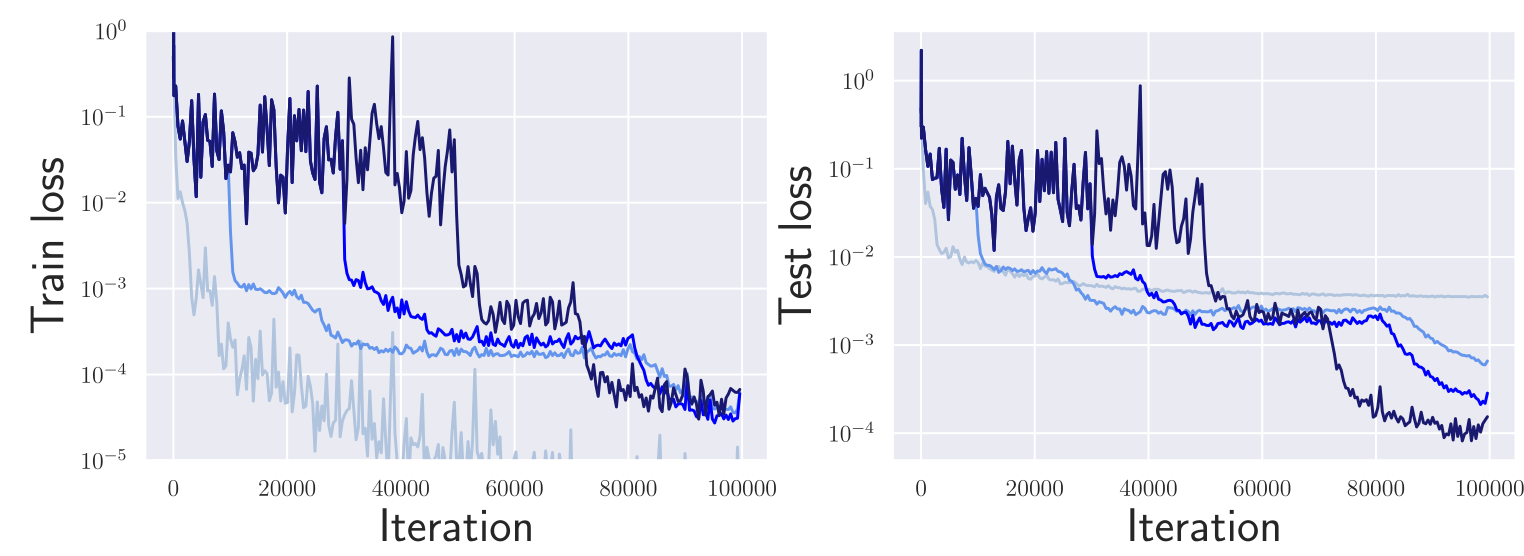
\includegraphics[width=0.8\textwidth,
            height=0.4\textheight]{./pics/dn_loss.png}
            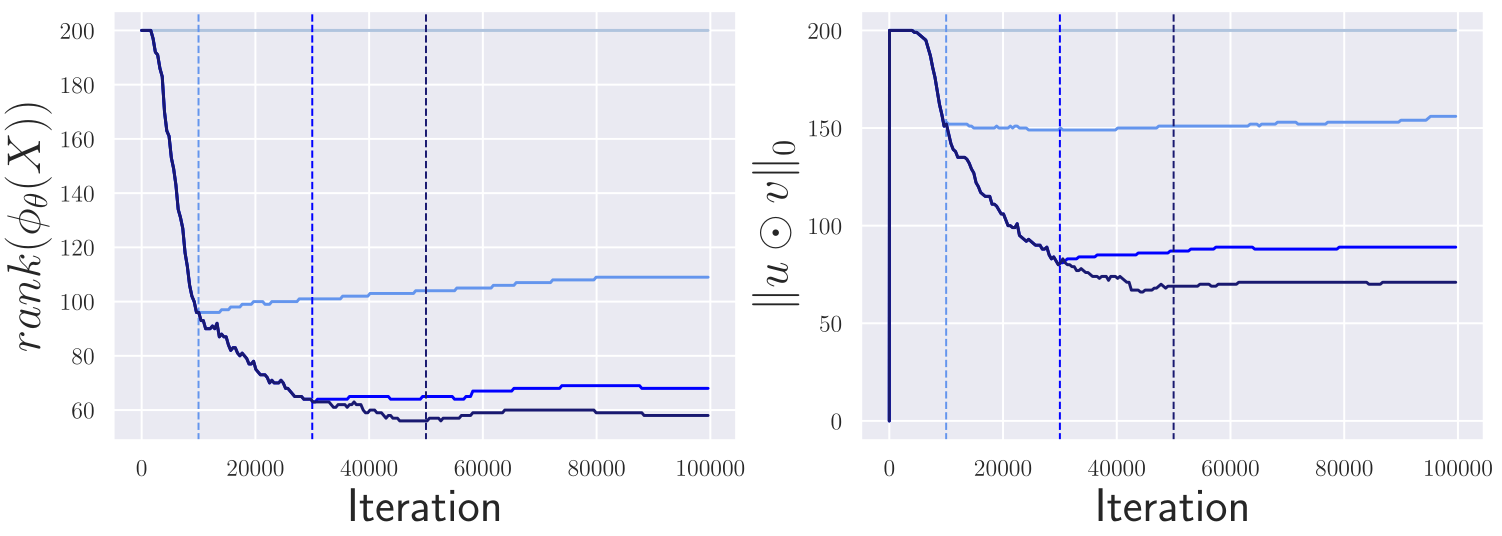
\includegraphics[width=0.8\textwidth,
            height=0.4\textheight]{./pics/dn_sparsity.png}
            
\includegraphics[width=\textwidth]{./pics/dn_setup.png}
            \caption{Diagonal Linear Nets Results}
        \end{figure}
    \end{frame}

    \begin{frame}{ReLU networks}
        \begin{itemize}
            \item \textbf{Two Layer} ReLU Setup: 1D regression task with 12 points
            \item SGD with $100$ neurons
            \item Similar results are observed
        \end{itemize}

        \begin{itemize}
            \item \textbf{Three Layer} ReLU Setup: teacher-student Setup
            \item Two neurons on each layer.
            \item Student network with $10$ neurons trained on $50$ samples
            \item Warm up step size (increasing step size according to a
                schedule)
        \end{itemize}
    \end{frame}

    \begin{frame}{ReLU Results}
        \begin{figure}[htpb]
            \centering
            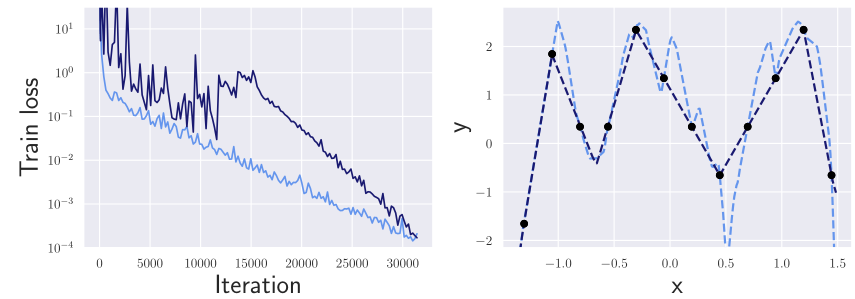
\includegraphics[width=0.8\textwidth,
            height=0.4\textheight]{./pics/relu2_loss.png}
            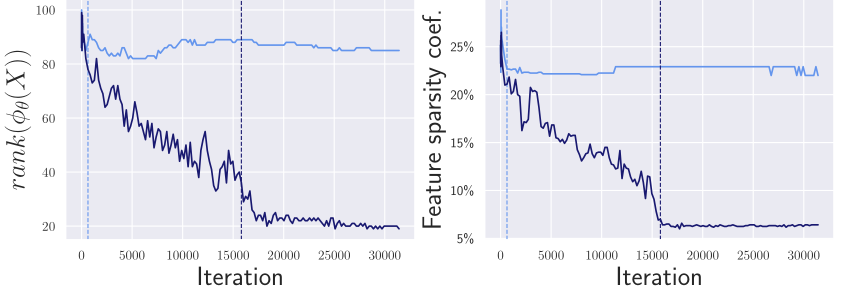
\includegraphics[width=0.8\textwidth,
            height=0.4\textheight]{./pics/relu2_sparsity.png}
            
\includegraphics[width=\textwidth]{./pics/relu2_setup.png}
            \caption{\textbf{Two Layer} ReLU: 1D regression task}
        \end{figure}
    \end{frame}

    \begin{frame}{ReLU Results}
        \begin{figure}[htpb]
            \centering
            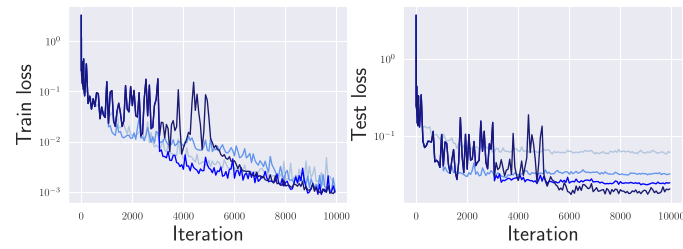
\includegraphics[width=0.8\textwidth,
            height=0.4\textheight]{./pics/relu3_loss.png}
            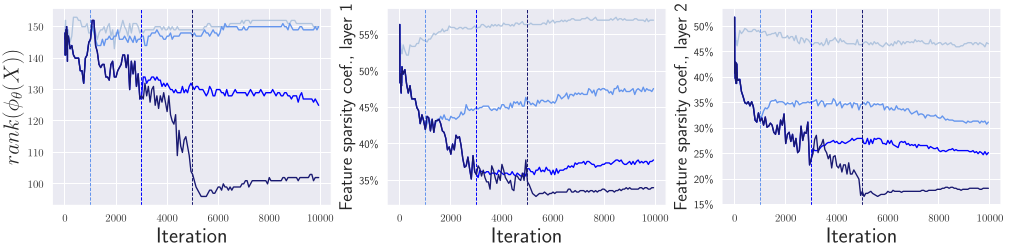
\includegraphics[width=\textwidth,
            height=0.4\textheight]{./pics/relu3_sparsity.png}
            
\includegraphics[width=\textwidth]{./pics/relu3_setup.png}
            \caption{\textbf{Three Layer} ReLU: teacher-student setup}
        \end{figure}
    \end{frame}

   \begin{frame}{Deeper Networks: Results}
        \begin{figure}[htpb]
            \centering
            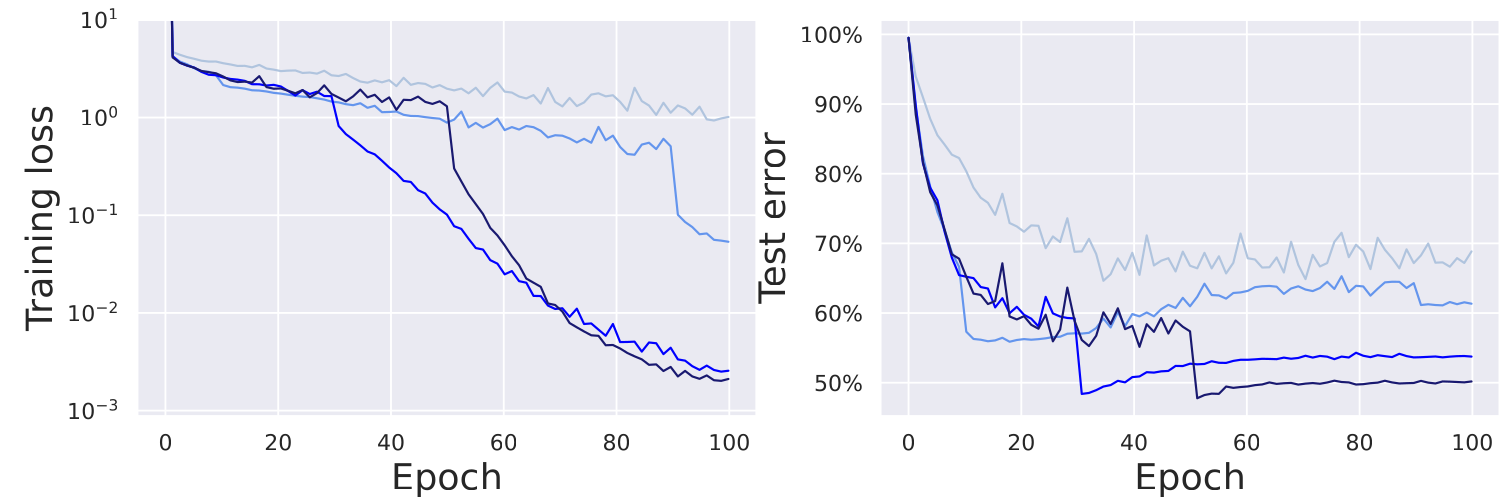
\includegraphics[width=0.8\textwidth,
            height=0.4\textheight]{./pics/densen_tiny_loss.png}
            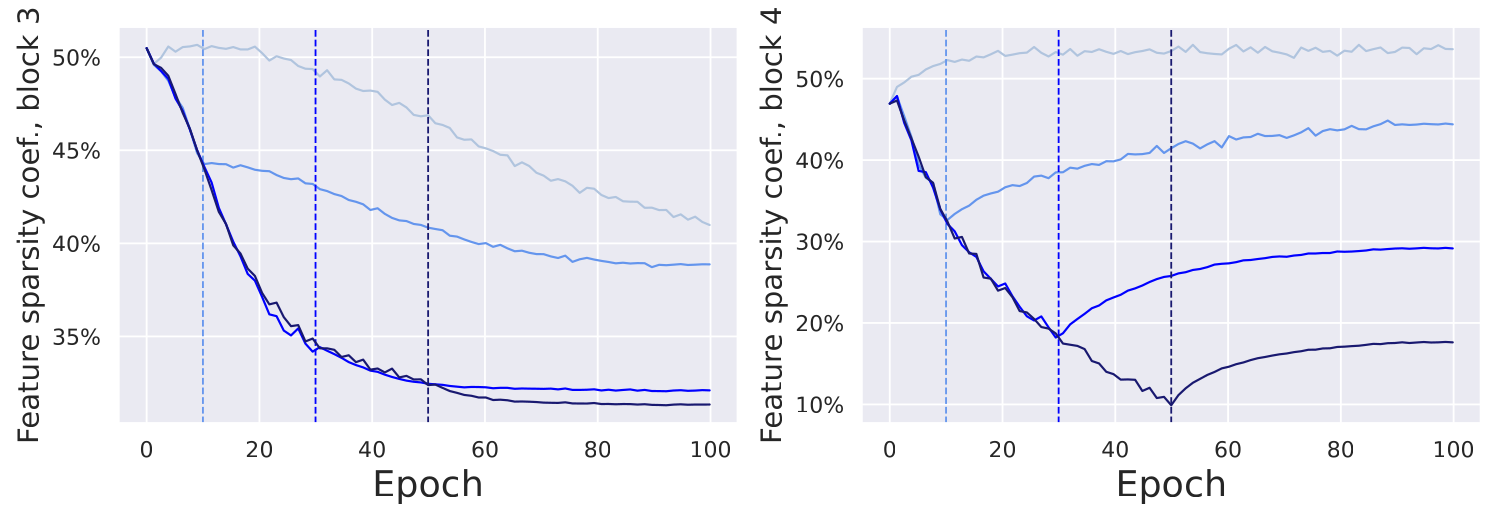
\includegraphics[width=0.8\textwidth,
            height=0.4\textheight]{./pics/densen_tiny_sparsity.png}
            
\includegraphics[width=\textwidth]{./pics/densen_tiny_setup.png}
            \caption{\textbf{DenseNet-100} trained on \textbf{ImageNet}
            (Image classification Task)}
        \end{figure}
   \end{frame}

\begin{frame}{Bibliography}
        \nocite{andriushchenko2023sgd}
        \nocite{shalev2014understanding}
        \nocite{li2018stochastic}
        \nocite{pillaudvivien2022label}
        \printbibliography
    \end{frame}
\end{document}
